%!LW recipe=latexmk-xelatex
\documentclass[handout,compress]{beamer}

\usetheme[block=fill]{metropolis}

\usepackage{graphicx} % Allows including images
\usepackage{amsmath,amsfonts,amsthm,amssymb}
\usepackage{color}
\usepackage{xcolor,cancel}
\usepackage{enumitem}
\setitemize{label=\usebeamerfont*{itemize item}%
	\usebeamercolor[fg]{itemize item}
	\usebeamertemplate{itemize item}}
\definecolor{mDarkBrown}{HTML}{604c38}
\definecolor{mDarkTeal}{HTML}{23373b}
\definecolor{mLightBrown}{HTML}{EB811B}
\definecolor{mMediumBrown}{HTML}{C87A2F}
\definecolor{mygreen}{HTML}{98C2B9}
\definecolor{myyellow}{HTML}{DFD79C}
\definecolor{myblue}{HTML}{8CA7CC}
\definecolor{kern}{HTML}{8CC2B7}


\usepackage{float}
\usepackage{framed}
\usepackage{epsfig}
\usepackage{graphicx}
\usepackage{subcaption}
\usepackage{ulem}
\usepackage{hhline}
\usepackage{multirow}
\usepackage{comment}   
\usepackage{bbm}
\usepackage{tikz}   
\def\Put(#1,#2)#3{\leavevmode\makebox(0,0){\put(#1,#2){#3}}}
\newcommand*\mystrut[1]{\vrule width0pt height0pt depth#1\relax}
\newcommand{\eqdef}{\mathbin{\stackrel{\rm def}{=}}}


\newcommand{\bs}[1]{\boldsymbol{#1}}
\newcommand{\bv}[1]{\mathbf{#1}}
\newcommand{\R}{\mathbb{R}}
\newcommand{\E}{\mathbb{E}}
\newcommand{\blue}[1]{\textcolor{blue}{#1}}

\DeclareMathOperator*{\argmin}{arg\,min}
\DeclareMathOperator*{\argmax}{arg\,max}
\DeclareMathOperator{\nnz}{nnz}
\DeclareMathOperator{\Var}{Var}
\DeclareMathOperator{\sinc}{sinc}
\DeclareMathOperator{\mv}{mv}
\DeclareMathOperator{\sgn}{sgn}
\DeclareMathOperator{\step}{step}
\DeclareMathOperator{\gap}{gap}
\DeclareMathOperator{\poly}{poly}
\DeclareMathOperator{\tr}{tr}
\DeclareMathOperator{\orth}{orth}
\newcommand{\norm}[1]{\|#1\|}
\captionsetup[subfigure]{labelformat=empty}
\captionsetup[figure]{labelformat=empty}
\DeclareMathOperator*{\lmin}{\lambda_{min}}
\DeclareMathOperator*{\lmax}{\lambda_{max}}

\newcommand{\specialcell}[2][c]{%
  \begin{tabular}[#1]{@{}c@{}}#2\end{tabular}}
\newcommand{\specialcellleft}[2][c]{%
\begin{tabular}[#1]{@{}l@{}}#2\end{tabular}
}

\usepackage{tabstackengine}
\stackMath


%----------------------------------------------------------------------------------------
%	TITLE PAGE
%----------------------------------------------------------------------------------------

\title{CS-GY 6763: Lecture 2 \\ Hashing + Fingerprinting, Chebyshev's Inequality}
\author{NYU Tandon School of Engineering, Prof. Christopher Musco}
\date{}

\begin{document}

\begin{frame}
	\titlepage 
\end{frame}

\metroset{titleformat=smallcaps}

\begin{comment}
\end{comment}

\begin{frame}
	\frametitle{note on mathematical proofs}
	\small
	It can be hard to know how formal to be. We will try to provide feedback on first problem set for anyone who is either too rigorous or too loose. It's a learning process.
	
	\textbf{Things that are generally fine:}
	\begin{itemize}
		\item Can assume input size $n$ is $> C$ for some constant $c$. E.g. $n > 2, n> 10$.
		\item Similarly can assume $\epsilon < c$ for constant $c$. E.g. $\epsilon < .1$, $\epsilon < .01$.
		\item If I write $O(z)$, you are free to choose the constant. E.g., it's fine if your analysis of CountSketch only works for tables of size $1000\cdot m$. 
		\item Derivatives, integrals, etc. can be taken from e.g. WolframAlpha without working through steps.
		\item Basic inequalities can be used {without proof}, as long as you verify numerically. Don't need to include plot on problem set.
	\end{itemize}
\end{frame}

\begin{frame}
	\frametitle{example inequality}
	\begin{align*}
		1+\epsilon \leq \frac{1}{1-\epsilon} \leq 1+ 2\epsilon \text{ for } \epsilon \in [0,.5].
	\end{align*}
\textbf{Proof by plotting:}
\begin{center}
	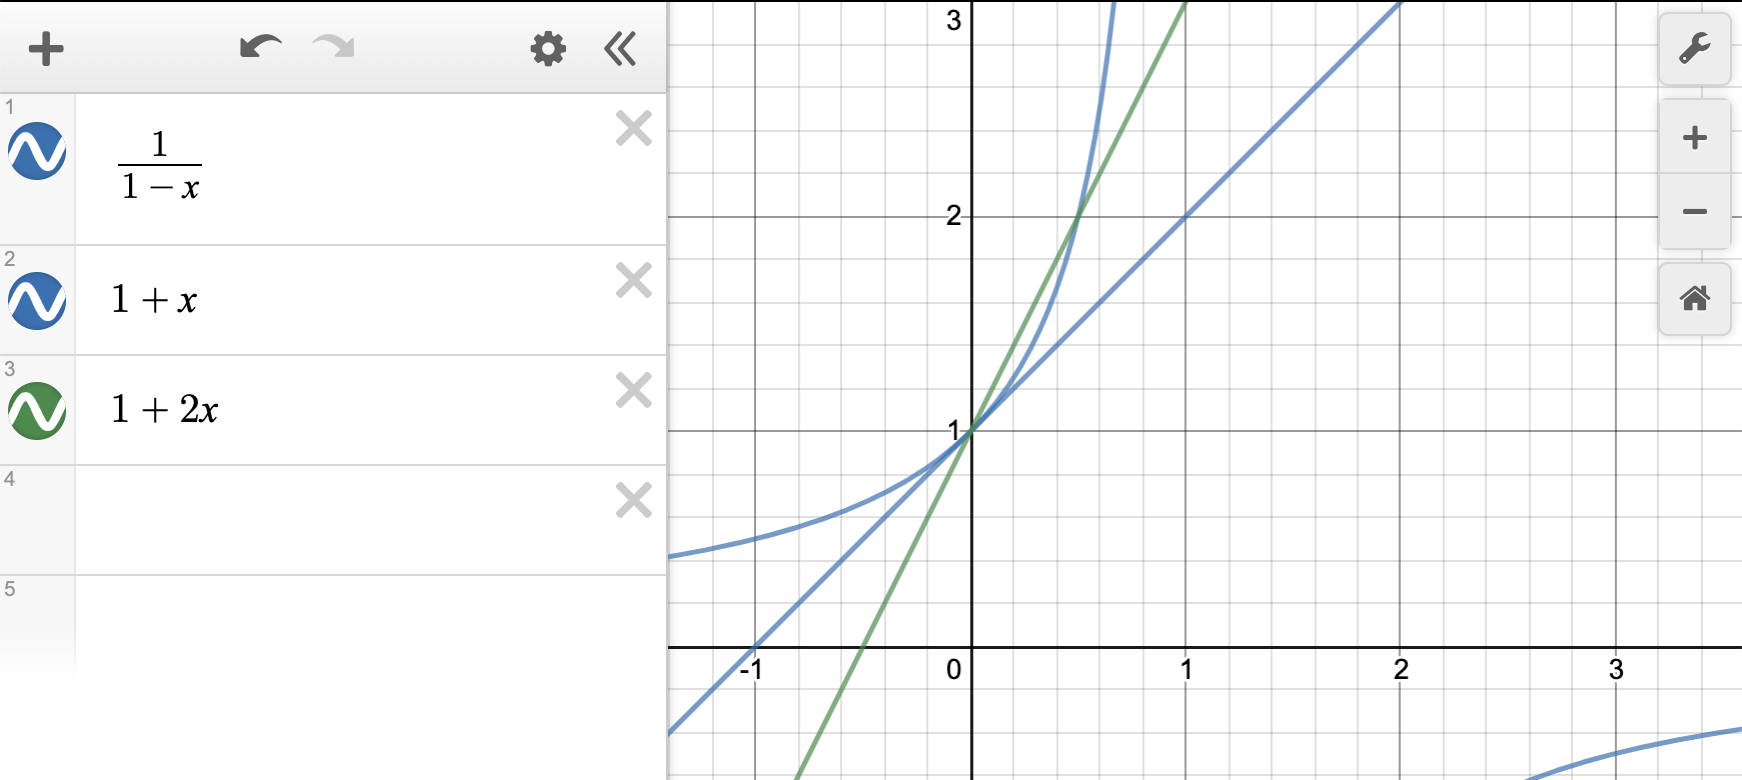
\includegraphics[width=\textwidth]{proof1.png}
\end{center}
\end{frame}

\begin{frame}
	\frametitle{example inequality}
	\begin{align*}
		1-\epsilon \leq \frac{1}{1+\epsilon} \leq 1 - .5\epsilon \text{ for } \epsilon \in [0,1].
	\end{align*}
	\textbf{Proof by plotting:}
	\begin{center}
		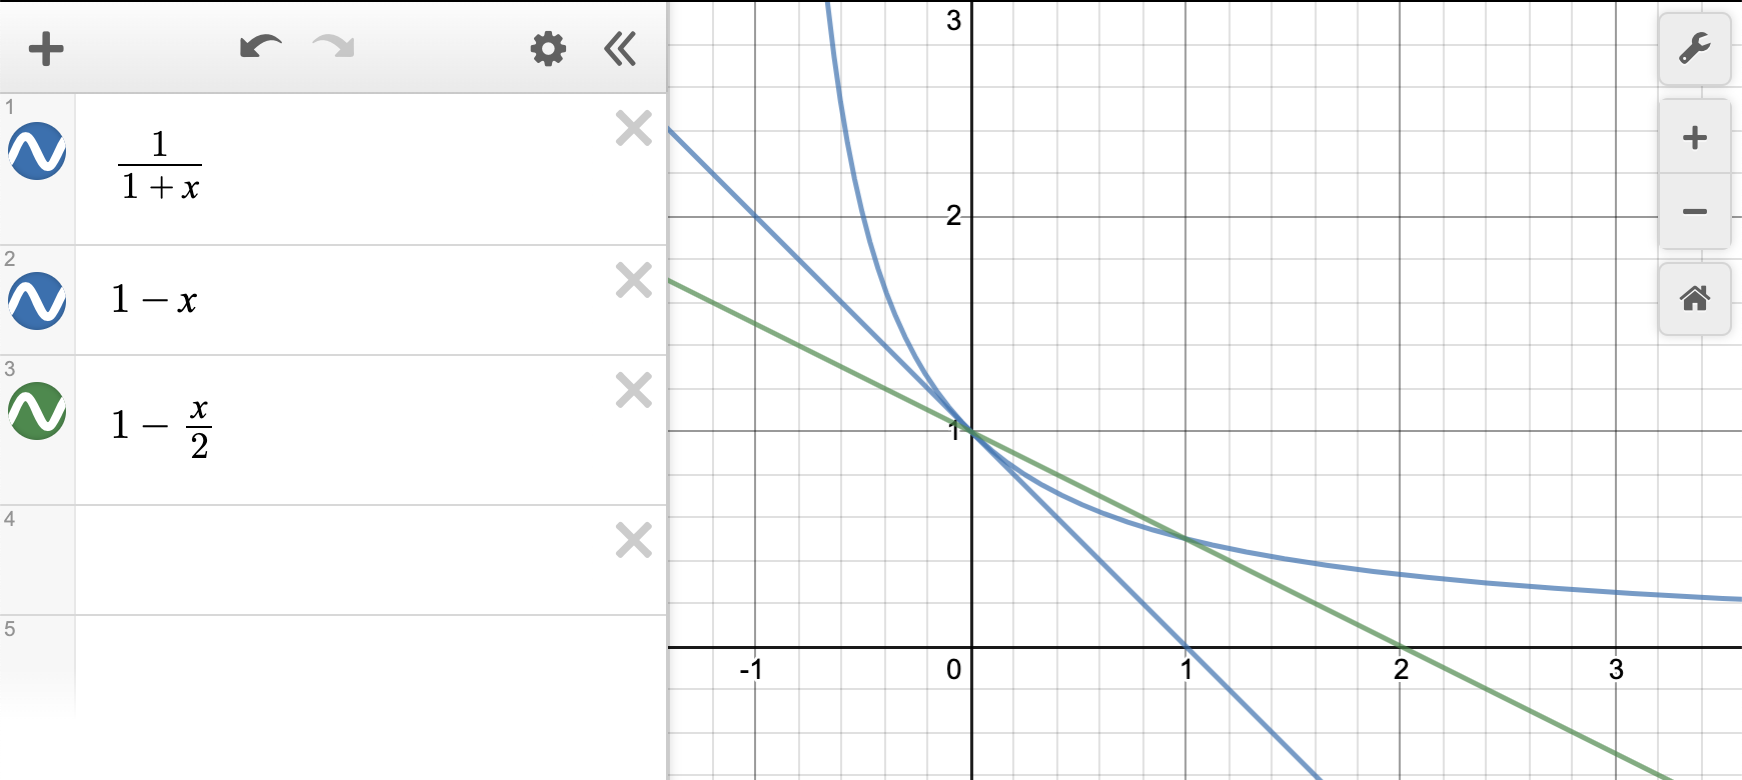
\includegraphics[width=\textwidth]{proof2.png}
	\end{center}
\end{frame}

\begin{frame} 
	\frametitle{general advice}
	\small
	\textbf{Tip:} When confronted with a complex expression, try to simplify by using big-Oh notation, or just rounding things off. Then clean-up your proof after you get to a solution.
	
	\textbf{Examples:}
	\begin{itemize}
		\item To start: $(m-1) \approx m$. \hspace{2.9em}Later: $m/2 \leq m-1 \leq m$. 
		\item To start: $\frac{1}{n} - \frac{1}{n^2} \approx \frac{1}{n}$. \hspace{3.5em}Later: $\frac{1}{2n} \leq \frac{1}{n} - \frac{1}{n^2} \leq \frac{1}{n}$.
		\item $\log(n/2)\approx \log(n)$
		\hspace{5em}Later: $\log(n)/2 \leq \log(n/2) \leq\log(n)$.
	\end{itemize}
\end{frame}

\begin{frame}
	\frametitle{definitions of independence}
	Suppose we have random variables $X_1, \ldots, X_k$. We say that \textbf{a pair of random variables} $X_i$ and $X_j$ are \emph{independent} if, for all possible values $v_i, v_j$,
	\begin{align*}
			\Pr[X_i = v_i \text{ and } X_j = v_j] = 	\Pr[X_i = v_i]\cdot \Pr[X_j = v_j].
	\end{align*}
	We say $X_1, \ldots, X_k$ are \emph{pairwise independent} if $X_i,X_j$ are independent for all $i,j \in \{1, \ldots, k\}$.

\vspace{1em}
We say $X_1, \ldots, X_k$ are \emph{mutually independent} if, for all possible values $v_1, \ldots, v_k$,
		\begin{align*}
			\Pr[X_1 = v_1, \ldots, X_k = v_k] = 	\Pr[X_1 = v_1]\cdot\ldots \cdot\Pr[X_k = v_k].
		\end{align*}
	
	Mutual independence implies pairwise independence, but pairwise independence does not imply mutual independence. 
\end{frame}

\begin{frame}[t]
	\frametitle{definitions of independence}
		\begin{center}
		\textbf{\alert{Give an example of three random variables that are pairwise independent but not mutually independent.}}
	\end{center}
	 $X_1, \ldots, X_k$ are \emph{pairwise independent} if for all $i,j$, $v_i, v_j$, 
	 \begin{align*}
	 	\Pr[X_i = v_i \text{ and } X_j = v_j = 	\Pr[X_i = v_i]\cdot \Pr[X_j = v_j].
	 \end{align*}
 	$X_1, \ldots, X_k$ are \emph{mutually independent} if, for all $v_1, \ldots, v_k$,
	\begin{align*}
		\Pr[X_1 = v_1, \ldots, X_k = v_k] = 	\Pr[X_1 = v_1]\cdot\ldots \cdot\Pr[X_k = v_k].
	\end{align*}
\end{frame}

\begin{frame}[t]
	\frametitle{linearity of variance}
	If we have two independent random variables $X,Y$, then:
	\begin{align*}
	\Var[X + Y] = \Var[X] + \Var[Y].
	\end{align*}
	\vspace{4.5em}

	If we have a set of pairwise independent\footnote{Technically, pairwise uncorrelated suffices, which is a weaker assumption.} random variables $X_1, \ldots, X_k$ then:\vspace{-1em}
	\begin{align*}
		\Var\left[\sum_{i=1}^k X_i\right] = \sum_{i=1}^k\Var[X_i].
	\end{align*}
	\begin{center}
	\textbf{\alert{Mutual independence is not necessary!}}\vspace{1em}
	\end{center}
\end{frame}



	\begin{frame}
		\frametitle{uniformly random hash function}
		Let $h$ be a \emph{random function} from $|\mathcal{U}| \rightarrow \{1,\ldots, m\}$. This means that $h$ is constructed by an algorithm using a seed of random numbers, but then the function is fixed. Given input $x\in \mathcal{U}$, it always returns the same output, $h(x)$. 
	
	\textbf{Recall: Uniformly Random Hash Function.} 
	A random function $h: \mathcal{U}\rightarrow \{1, \ldots, m\}$ is called uniformly random if:
	\begin{itemize}
		\item $\Pr[h(x) = i] = \frac{1}{m}$ for all $x\in \mathcal{U}$, $i\in \{1,\ldots, m\}$.  
		\vspace{.5em}
		\item $h(x), h(y), h(z), \ldots$ are mutually independent random variables for all $x,y,z, \ldots \in \mathcal{U}$. 
		\begin{itemize}
			\vspace{.5em}
			\item Which implies that $\Pr[h(x) = h(y)] = $ \vspace{2em}
			\item Which implies that $\Pr[h(x) = h(y) = h(z)] = $ 

		\end{itemize}
	\end{itemize}
	
	\vspace{2em}
	\begin{block}{\vspace*{-3ex}}
		\small $\mathcal{U} = $ universe of possible keys, $m=$ number of values hashed to.
	\end{block}
\end{frame}

	\begin{frame}[t]
	\frametitle{uniformly random hash function}
	\begin{center}
	The only way to implement a \emph{truly} random hash function is to create a giant lookup table, where the numbers on the right are chosen independently at random from $\{1, \ldots, m\}$. 
	
		\begin{tabular}{c | c } 
		x & h(x) \\
		\hline 
		1 & 14\\ 
		2 & 25\\ 
		3 & 99\\ 
		4 & 16\\ 
		$\vdots$ & $\vdots$\\
		$|\mathcal{U}|$ & 87
		\end{tabular}
	\end{center}
If we're hashing 35 char ASCII strings (e.g. urls) the length of the table is \emph{greater than the number of atoms in the universe.}
	\end{frame}

	\begin{frame}[t]
	\frametitle{universal hash functions}
	For the application to CountMin from last class we can weaken our assumption that $h$ is uniformly random.
	\begin{definition}[Universal hash function]
		A random hash function $h: \mathcal{U} \rightarrow \{1, \ldots, m\}$ is \emph{universal} if, for any fixed $x,y\in \mathcal{U}$,
		\begin{align*}
			\Pr[h(x) = h(y)] \leq \frac{1}{m}.
		\end{align*}
	\end{definition}
	\textbf{Claim:} A uniformly random hash-function is universal. 

\end{frame}

	\begin{frame}
		\frametitle{universal hash functions}
		\begin{definition}[Universal hash function]
		A random hash function $h: \mathcal{U} \rightarrow \{1, \ldots, m\}$ is \emph{universal} if, for any fixed $x,y\in \mathcal{U}$,\vspace{-1.5em}
		\begin{align*}
			\Pr[h(x) = h(y)] \leq \frac{1}{m}.
		\end{align*}
	\end{definition}
	\textbf{Efficient alternative:} Let $p$ be a prime number between $|\mathcal{U}|$ and $2|\mathcal{U}|$. Let $a,b$ be random numbers in $0,\ldots, p$, $a\neq 0$.
	\begin{align*}
		h(x) = \left[a\cdot x + b \pmod{p}\right] \pmod{m}
	\end{align*} 
	is universal. Lecture notes with proof posted on website. Requires some abstract algebra.
	
	\begin{center}
	\textbf{How much space does this hash function take to store?}
	\end{center}
\end{frame}

\begin{frame}[t]
	\frametitle{limited independence hash functions}
Similar alternative definition:
	\begin{definition}[Pairwise independent hash function]
		A random hash function $h: \mathcal{U} \rightarrow \{1, \ldots, m\}$ is pairwise independent if, for any fixed $x,y\in \mathcal{U}, i,j \in \{1\ldots, m\}$,
		\begin{align*}
			\Pr[h(x) = i \text{ and } h(y) = j] = \frac{1}{m^2}.
		\end{align*}
	\end{definition}
Basically same construction as universal hash, except we don't restrict $a \neq 0$ and $m$ to be a prime power.

\textbf{Claim:} A pairwise independent hash-function is universal. 

\end{frame}

\begin{frame}[t]
	\frametitle{limited independence hash functions}
	\begin{definition}[$k$-wise independent hash function]
		A random hash function $h: \mathcal{U} \rightarrow \{1, \ldots, m\}$ is $k$-wise independent if, for any fixed $x,y\in \mathcal{U}, i,j \in \{1\ldots, m\}$,
		\begin{align*}
			\Pr[h(u_1) = v_1 \text{ and } h(u_2) = v_2 \text{ and } \ldots h(u_k) = v_k] = \frac{1}{m^k}, 	
		\end{align*}
		for all $u_1, \ldots, u_k \in \mathcal{U}$ and $v_1, \ldots, v_k \in \{1, \ldots, m\}$.
	\end{definition}

Strictly stronger than pairwise independence and needed for some applications. But we will never need $k > O(\log n)$ in this class. 

\textbf{Example:} For random coefficients $c_0, \ldots, c_k \in \{0, \ldots, p\}$,
\begin{align*}
	h(x) = \left[c_0 + c_1 x + c_2 x^2 + \ldots c_k x^k \pmod{p}\right] \pmod{m}
\end{align*}
\end{frame}



\begin{frame}
	\frametitle{pseudorandom hash functions}
	We won't prove that random polynomials provide good hash functions, but I want to give a flavor of what is involved (e.g., why do prime numbers show up?).
\end{frame}

\begin{frame}
	\frametitle{fingerprinting}
	\textbf{Goal:} Construct a compact ``fingerprint'' $h(f)$ for any given file $f$ with two properties:
	\begin{itemize}
		\item The fingerprints $h(f_1)$ and $h(f_2)$ should be different with high probability if the contents of $f_1$ and $f_2$ differ at all. 
		\item If the contents of $f_1$ and $f_2$ are identical, we should have $h(f_1) = h(f_2)$.
	\end{itemize}
	\begin{center}
		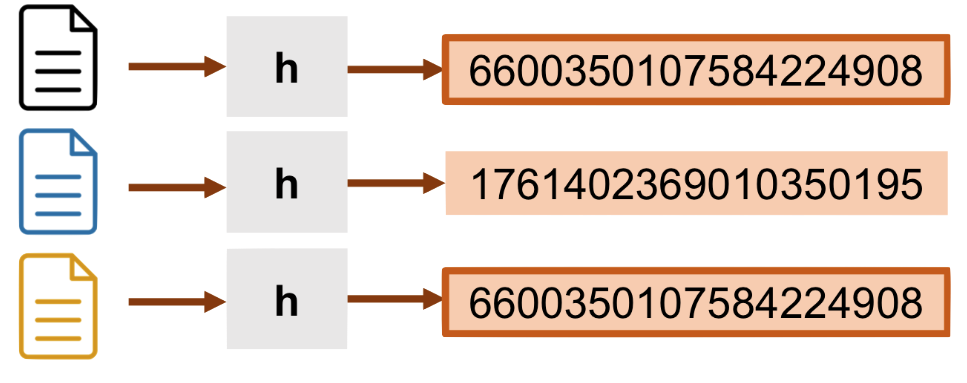
\includegraphics[width=.75\textwidth]{finger_print.png}
	\end{center}
	\begin{center}
	(Basically the same goal as most applications of hashing.)
	\end{center}
\end{frame}

\begin{frame}[t]
	\frametitle{applications of finger printing}
	\begin{itemize} 
		\item Quickly check if two versions of the same file are identical (e.g. in version control systems like Git). Do not need to communicate the entire file between servers. Also used in webcaching and content delivery networks. 
		\item Check that a file pieced together from multiple parts is not missing anything. 
	\end{itemize}
	
\end{frame}

\begin{frame}[t]
	\frametitle{applications of finger printing}
	\begin{center}
		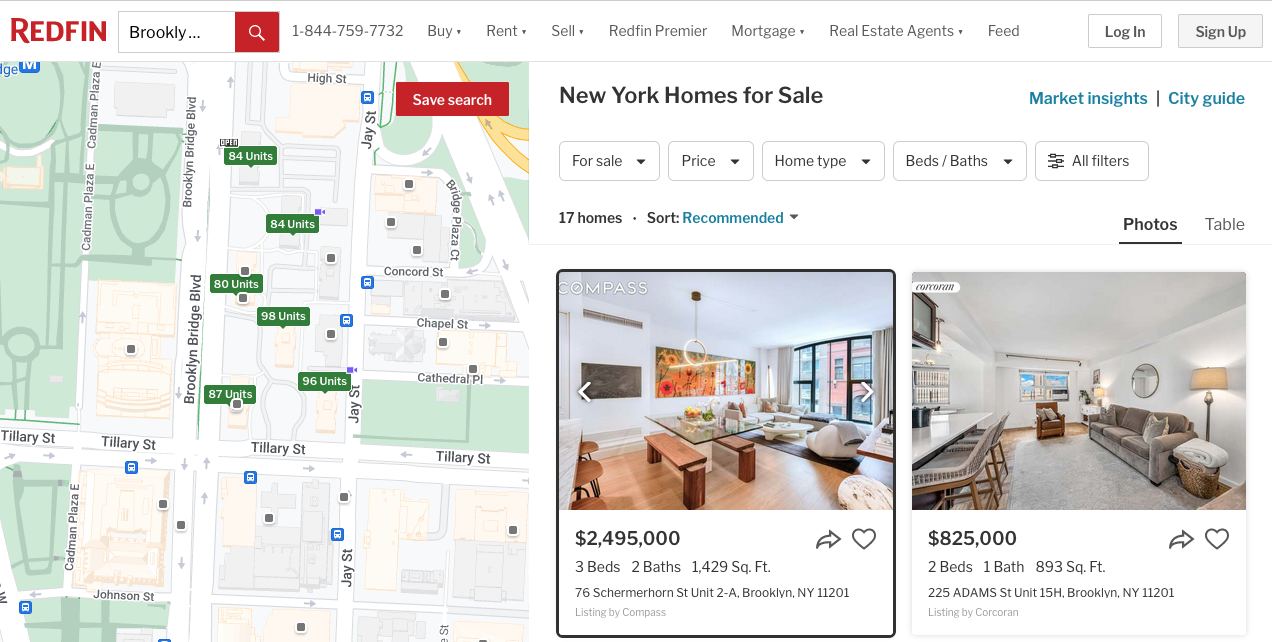
\includegraphics[width=\textwidth]{redfin_1.png}
	\end{center}
\end{frame}

\begin{frame}[t]
	\frametitle{applications of finger printing}
	\begin{center}
		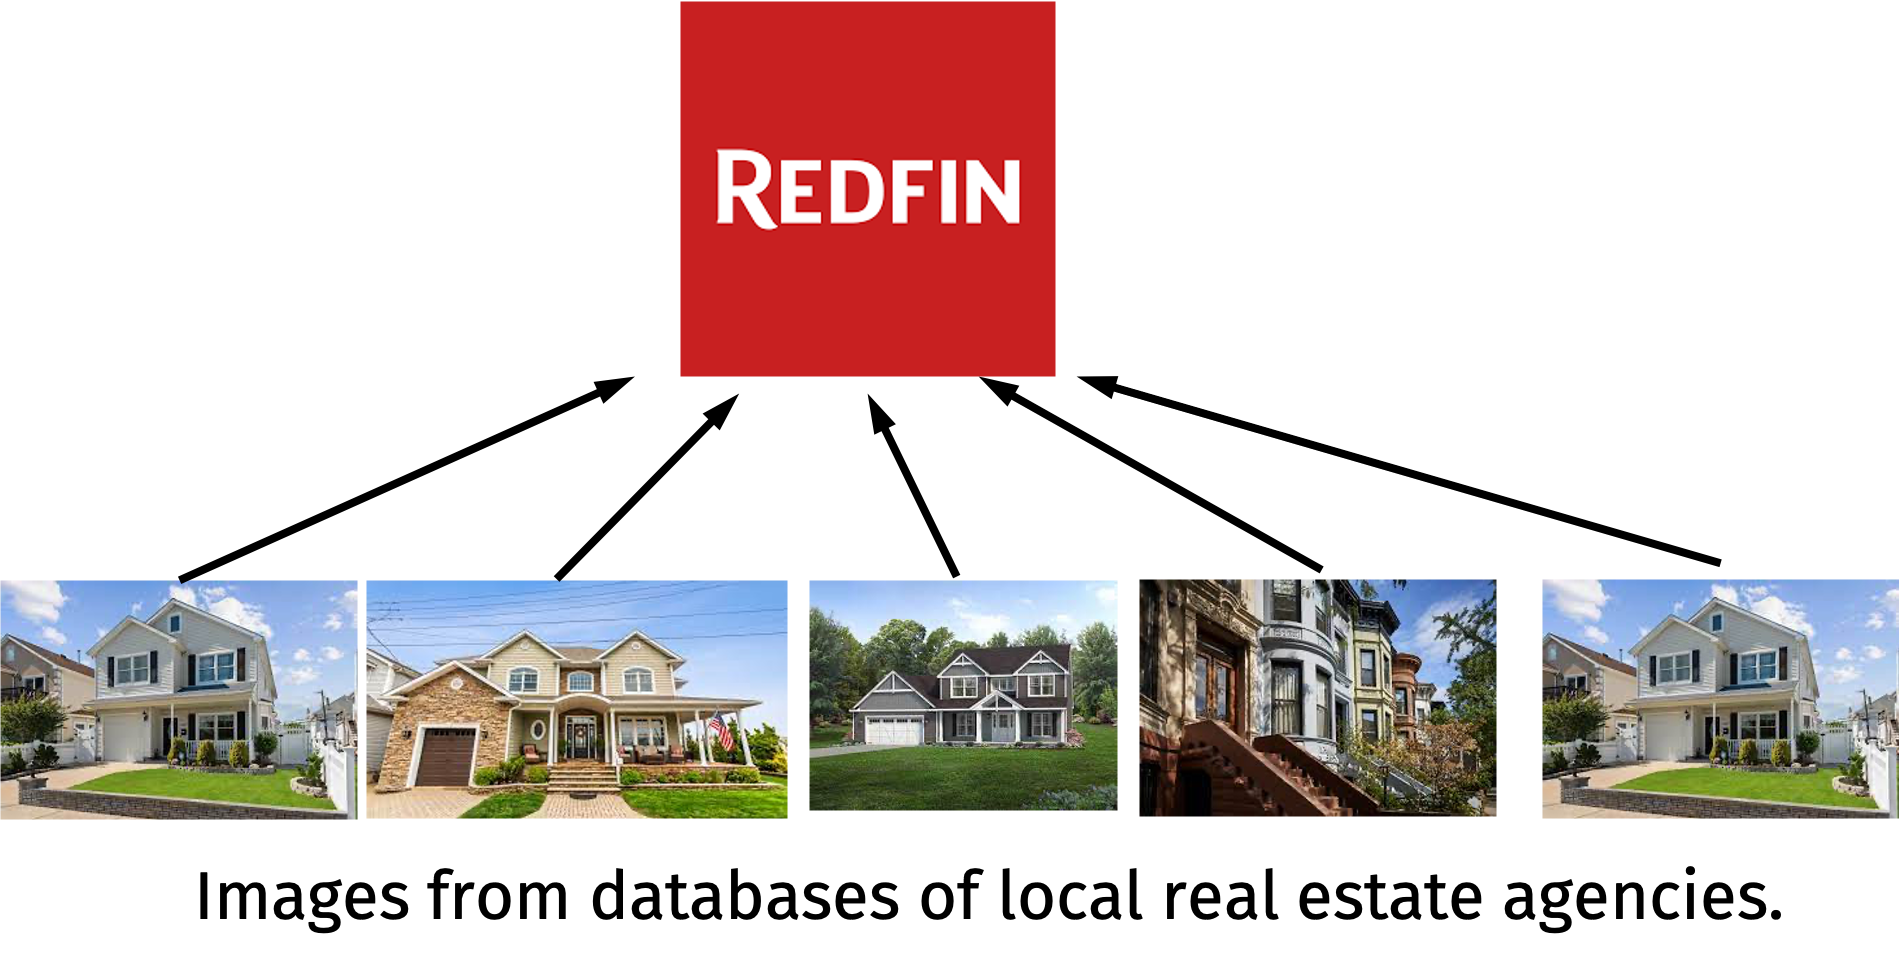
\includegraphics[width=\textwidth]{redfin_2.png}
	\end{center}
	
	Fingerprints used as file names for the images to make sure we did not reupload new images that we already had, and to detect duplicate images and listings.
\end{frame}

\begin{frame}
	\frametitle{fingerprinting}
	\textbf{Goal:} Construct a compact ``fingerprint'' function $h(f)$ such that:
	\begin{itemize}
		\item $h(f_1) \neq h(f_2)$ if $f_1 \neq f_2$ with high probability.
	\end{itemize}
\vspace{1em}
	Ideally, length of $h(f_1)$ (i.e. the size of the integers hashed to) is much less than the file size. 
\end{frame}

\begin{frame}
	\frametitle{random fingerprinting}
	\textbf{Rabin Fingerprint (1981)}: Let file $f = 010\ldots1101$ of length $n$ be interpreted as an $n$ bit integer. So something between $0$ and $2^n$. 
	
	\textbf{Construct $h$ randomly:} Choose random prime number $p$  between $2$ and $tn\log(tn)$ for a constant $t$.
	\begin{align*}
		h(f) = f \pmod{p}.
	\end{align*} 
	
	\begin{center}
		How many bits does $h(f)$ take to store?
	\end{center}
	
\end{frame}

\begin{frame}[t]
	\frametitle{random fingerprinting}
	\begin{align*}
		h(f) = f \pmod{p} \text{\hspace{1em} for random prime } p\in \{2, \ldots, tn\log(tn)\}
	\end{align*} 
	\textbf{Claim:} If $f_1\neq f_2$ then $h(f_1) = h(f_2)$ with probability  $\leq \frac{2}{t}$.
	\vspace{3em}
	
	Since our fingerprint only takes $O(\log n + \log t)$ space,   we can  set $t$ to be \emph{super large}, so effectively the probability of $h(f_1)$ and $h(f_2)$ colliding is negligible for all real-world applications.
	
	E.g. set fingerprint length to $\log n + 28$ bits and you are more likely to win Megamillions.
\end{frame}

\begin{frame}[t]
	\frametitle{random fingerprinting}
	How do we sample a random prime between $2,\ldots, tn\log n$?


	Keep in mind that $n$ is pretty large here. For a 200kb image, $n \approx 1.6$ million. 
\end{frame}

% \begin{frame}
% 	\frametitle{prime number checking}
% 	\begin{center}
% 		\textbf{\alert{One of the most famous applications of randomness in algorithm design.}}
% 	\end{center}
% 	\textbf{Computational Problem:} Given a number $x$, is $x$ prime? 
	
% 	\textbf{Recall:} 
% 	\begin{itemize}
% 		\item A number is prime if it can only be divided evenly by $1$ and itself. 
% 		\item The first few primes are $2,3,5,7,11,13, 17, 19,\ldots$.
% 		\item Is 2023 prime?
% 		\item What about 49301977064557719291?
% 	\end{itemize}
% 	\textbf{How would you design a generic algorithm to check?}
% \end{frame}

% \begin{frame}
% 	\frametitle{prime number checking}
% 	Suppose we have an integer represented as a length $n$ binary string. 
% 	\begin{align*}
% 		x = 0110100010110101\ldots1010001110
% 	\end{align*}
% The naive prime checking algorithm runs in $O(2^n)$ time. 

% NYU Greene Super Computer has $~ 2$ petaFLOPS of throughput. When $n = 128$, would need 1 million Greene Super computers running for 1 million years to check is $x$ is prime. 
% \end{frame}

% \begin{frame}
% 	\frametitle{randomized primality test}
% 	\textbf{Miller-Rabin 1976, 1980:} There is a \emph{randomized} algorithm running in $O(n^3 \log_2(1/\delta))$ time that, with probability $1-\delta$ determines if an $n$-bit integer $x$ is prime.  
% 	\begin{itemize}
% 		\item $n = 128$
% 		\item $\delta = 10^{-9}$ (chance of winning the Powerball Jackpot)
% 		\item $n^3\log_2(1/\delta) \approx 60$ million operations.
% 	\end{itemize}
% 	Could check in $< .1$ second on my laptop.
% 	\begin{center}
% 		\large \alert{\textbf{This was a really big break through!}}
% 	\end{center}
% \end{frame}

% \begin{frame}
% 	\frametitle{randomized primality test}
% 	Took over 20 more years to find a \emph{deterministic} polynomial time primality test.
% 	\begin{center}
% 		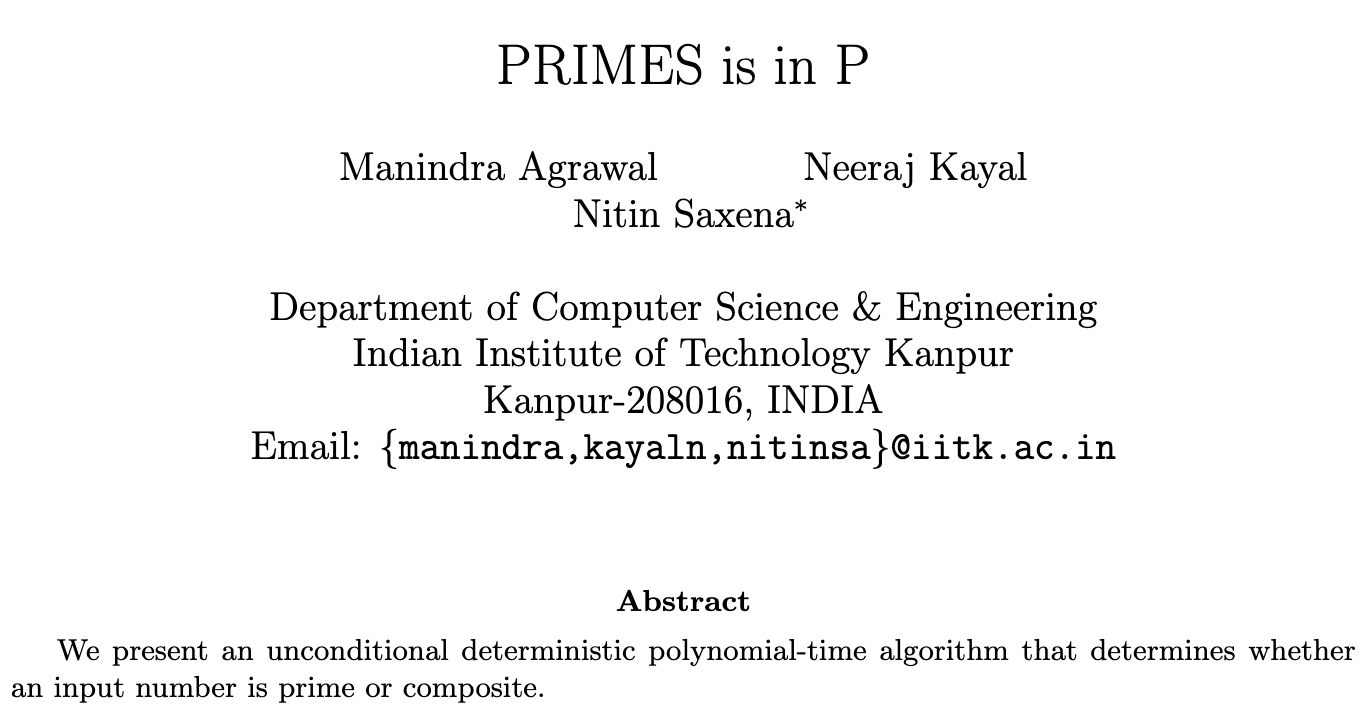
\includegraphics[width=\textwidth]{primes_in_p.png}
% 	\end{center}
% \end{frame}


\begin{frame}
	\frametitle{from prime testing to prime generation}
	\textbf{Rejection sampling:}
	\begin{itemize}
		\item Pick a random $q$ bit number. 
		\item Check if it's prime. Can be done in $O(q^3)$ time.
		\item If not, repeat.
	\end{itemize}
	Here we would have $q \approx \log(tn\log n) \approx 48$ for the example above. So each iteration is efficient, but is this efficient overall?
	\begin{center}
		\emph{Roughly how many tries do you expect this to take?}
	\end{center}
\end{frame}

\begin{frame}
	\frametitle{prime number theorem}
 Let $\pi(x)$ denote the number of primes less than some integer $x$. 	\textbf{Informally:}
	\vspace{-.5em}
	\begin{align*}
		\pi(x) \sim \frac{x}{\ln(x)}
	\end{align*}
	\vspace{-1em}
	
	\begin{center}
		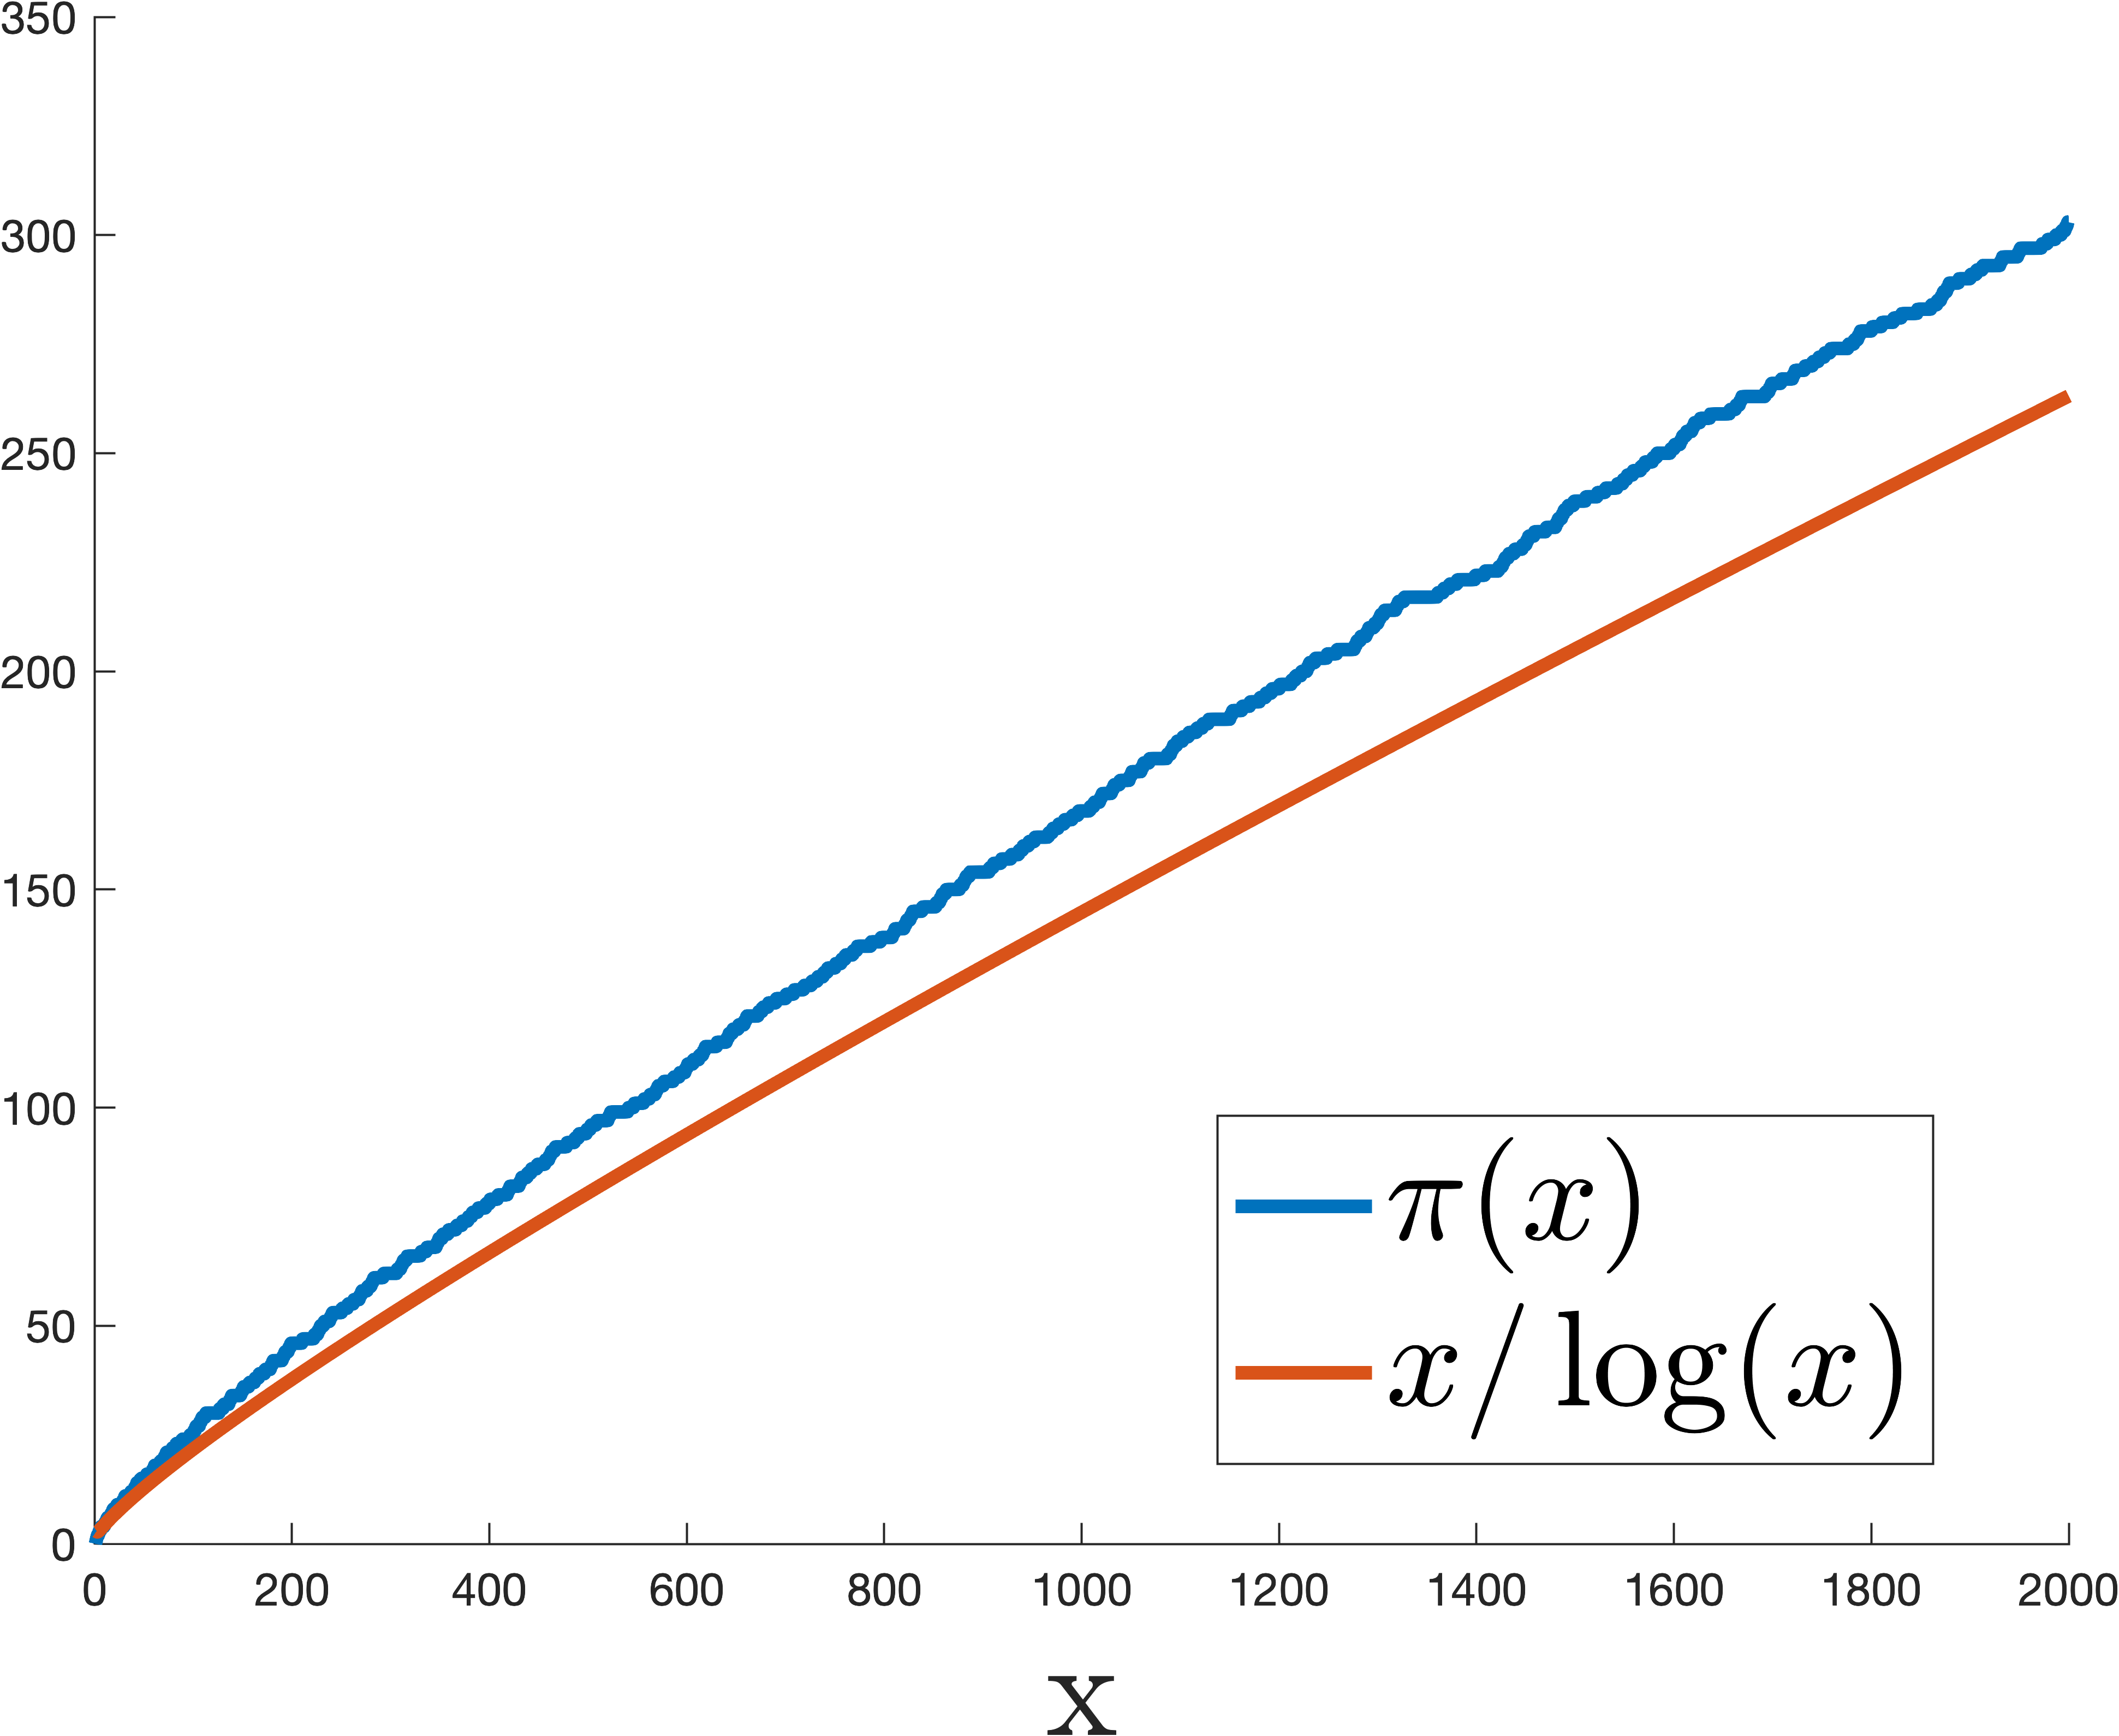
\includegraphics[width=.6\textwidth]{prime_number_theorem.png}
	\end{center}
\end{frame}

\begin{frame}
	\frametitle{prime number theorem}
	\textbf{Formally:}	For $x > 17$,
	\begin{align*}
		\frac{x}{\ln(x)} \leq	\pi(x) \leq \frac{x}{\ln(x) - 4}
	\end{align*}
	
	So if we select a random $q = 48$ bit number, the chance that it is prime is great than:
	\begin{align*}
		\frac{1}{\ln(2^{q})} \geq \frac{1}{34}
	\end{align*} 
	After a few hundred tries, we will almost definitely find a prime number. \textbf{In general, need $O(q)$ tries in expectation to find a prime with $q$ bits.}

	\textbf{Remark:} Finding large prime numbers is important in some other applications beyond hashing.
\end{frame}



\begin{frame}[t]
	\frametitle{random fingerprinting}
	\begin{align*}
		h(f) = f \pmod{p} \text{\hspace{1em} for prime } p\in \{2, \ldots, tn\log(tn)\}
	\end{align*} 
	\textbf{Claim:} If $f_1\neq f_2$ then $h(f_1) = h(f_2)$ with probability $\leq \frac{2}{t}$.
	\vspace{3em}
	
	\textbf{First observation:} If $h(f_1) = h(f_2)$, then:
	\begin{align*}
		(f_1 - f_2) \pmod{p} = 0. 
	\end{align*}
	In other words, we only fail  \emph{if $|f_1 - f_2|$ is divisible by $p$}.
	
	
\end{frame}

\begin{frame}[t]
	\frametitle{random fingerprinting}
	\textbf{Question:} What is the chance that $|f_1 - f_2|$ is divisible by a random prime $p\in \{2, \ldots, tn\log(tn)\}$?
	
\end{frame}

\begin{frame}[t]
	\frametitle{random fingerprinting}
	\textbf{Number of distinct prime factors of $f_1 - f_2$}: At most $n$.
	\vspace{1em}
	
	\textbf{Number of primes between $\{2, \ldots, tn\log(tn)\}$}: At least $\frac{tn\log(tn)}{\log(tn\log(tn))}$ via prime number theorem.
	
	\vspace{-.25em}
	\begin{center}
		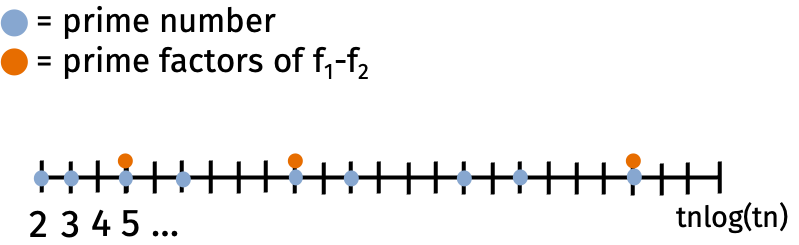
\includegraphics[width=.8\textwidth]{number_line.png}
	\end{center}
	\vspace{-.25em}
Chance we pick a prime factor of $f_1 - f_2$ is less than:
	\begin{align*}
		\frac{n}{\frac{tn\log(tn)}{\log(tn\log(tn))}} =  \frac{\log(tn\log(tn))}{t\log(tn)} \leq \frac{2\log(tn)}{t\log(tn)}
	\end{align*}	
	
\end{frame}


\begin{frame}[t]
	\frametitle{random fingerprinting}
	\textbf{Conclusion:} The chance that a \emph{random} prime $p\in \{2, \ldots, tn\log(tn)\}$ is a factor of $|f_1 - f_2|$ is $\leq \frac{2}{t}$.
	
	So, for two files $f_1 \neq f_2$, the chance that $h(f_1) = h(f_2) \leq \frac{2}{t}$.
	\vspace{2em}
	
	Set $t = 2^{28}$ (the chance you win Megamillions).
	
	\textbf{Fingerprint size:} At most $2\log_2(nt) = 2\log_2(n) + 2\log_2(2^{28})$ bits. 
	
	Suppose we are fingerprinting $200$kb image files. $n \approx 1,600,000$, so our fingerprint has size:
	\begin{align*}
		\alert{\mathbf{96}}\text{ \textbf{\alert{bits}}}
	\end{align*}
	
	This amounts to a \emph{17,000x reduction} over sending and comparing the original files.
\end{frame}



\begin{frame}
	\frametitle{remainder of lecture}
	Last week we saw the power of \emph{Linearity of Expectation} + \emph{Markov's}. This week we will discuss two more tools:
	\begin{itemize}
		\item \emph{Linearity of Variance} + \emph{Chebyshev's Inequality}
	\end{itemize}
	Next week:
	\begin{itemize}
	\item \emph{Union Bound} + \emph{Exponential Tail Bounds}
	\end{itemize}
	\begin{center}
		
\includegraphics[width=.5\textwidth]{4function.png}
		
		\textbf{\alert{These six tools combined are surprising powerful and flexible. They form the cornerstone of randomized algorithm design.}}
	\end{center}
 \end{frame}

\begin{frame}
	\frametitle{chebyshev's inequality}
	\small
	A new concentration inequality:
	\begin{lemma}[Chebyshev's Inequality]
		Let $X$ be a random variable with expectation $\E[X]$ and variance $\sigma^2 = \Var[X]$. Then for any $k > 0$,
		\begin{align*}
			\Pr[|X - \E[X]| \geq k\cdot\sigma] \leq \frac{1}{k^2}
		\end{align*}
	\end{lemma}
	\vspace{-.5em}
	\begin{center}
		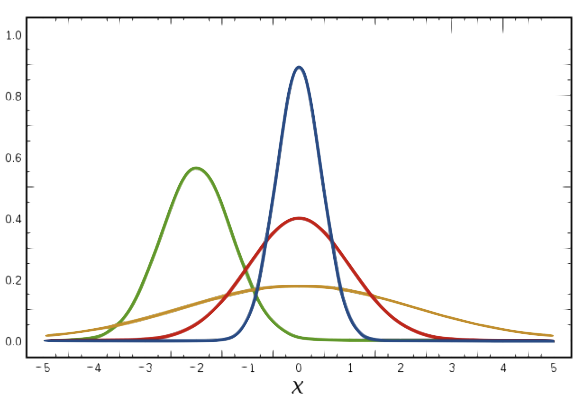
\includegraphics[width=.4\textwidth]{rvs.png}
		
		$\sigma = \sqrt{\Var[X]}$ is the \emph{standard deviation} of $X$. Intuitively this bound makes sense: it is {tighter} when $\sigma$ is smaller.
	\end{center}
	%\vspace{-2em}
	%	\begin{block}{\vspace*{-3ex}}
	%		\small
	%		Recall, $\Var[X] = \E[(X - \E[X])^2] = \E[X^2] - \E[X]^2$.
	%	\end{block}
\end{frame}

\begin{frame}
	\frametitle{comparison to markov's inequality}
	\small
	Properties of Chebyshev's inequality:
	\begin{itemize}
		\item \textbf{Good:} No requirement of non-negativity. $X$ can be anything.
		\item \textbf{Good:} Two-sided. Bounds the probability that $|X - \E X|$ is large, which means that $X$ isn't too far above \emph{or} below its expectation. Markov's only bounded probability that $X$ exceeds $\E[X]$.
		\item \textbf{Bad/Good:} Requires a bound on the variance of of $X$.  
	\end{itemize}
	\alert{\textbf{No hard rule for which to apply! Both Markov's and Chebyshev's are useful in different settings.}}
\end{frame} 

\begin{frame}
	\frametitle{proof of chebyshev's inequality}
	\small
	\textbf{Idea:} Apply Markov's inequality to the (non-negative) random variable $S = (X-\E[X])^2$.
	\begin{lemma}[Chebyshev's Inequality]
		Let $X$ be a random variable with expectation $\E[X]$ and variance $\sigma^2 = \Var[X]$. Then for any $k > 0$,
		\begin{align*}
			\Pr[|X - \E[X]| \geq k\cdot\sigma] \leq \frac{1}{k^2}
		\end{align*}
	\end{lemma}
%	\begin{align*}
%		\Pr[S \geq k^2\sigma^2] &\leq \frac{\E[S]}{k^2\sigma^2} \text{\hspace{2em}\blue{(Markov inequality)}}\\
%		\Pr[\sqrt{S} \geq k\sigma] &\leq \frac{\E[(X-\E[X])^2]}{k^2\sigma^2}\\
%		\Pr[|X - \E[X]|\geq k\sigma] &\leq \frac{\sigma^2}{k^2\sigma^2} = \frac{1}{k^2}.\qed
%	\end{align*}
	
	\vspace{7em}
	\begin{block}{\vspace*{-3ex}}
		\small \textbf{Markov's inequality}: for non-negative r.v. $S$, $\Pr[S \geq t] \leq \E[S]/t$.  
	\end{block}
\end{frame}

\begin{frame}
	\frametitle{quick example}
	\begin{center}
	\textbf{If I flip a fair coin $100$ times, show that with $> 93\%$ chance I get between $30$ and $70$ heads.}
	\end{center}
	Let $C_1, \ldots, C_{100}$ be independent random variables that are $1$ with probability $1/2$, $0$ otherwise.

	Let $H = \sum_{i=1}^{100} C_i$ be the number of heads that get flipped.	
	
	\begin{align*}
		\E[H] = \hspace{20em}
	\end{align*}

	\begin{align*}
	\Var[H] = \hspace{20em}
	\end{align*}
\vspace{4em}
\end{frame}

% \begin{frame}
% 	\frametitle{linearity of variance}
% 	\textbf{Recall:} For \emph{pairwise independent}\footnote{Technically, pairwise uncorrelated suffices, which is a slightly weaker assumption.} random variables $X_1, \ldots, X_m$, 
% 	\begin{align*}
% 		\Var[X_1 + X_2 + \ldots + X_m] = 	\Var[X_1]+ \Var[X_2] + \ldots + \Var[X_m]. 
% 	\end{align*}
% I.e., we require that for any $i,j$ $X_i$ and $X_j$ are independent. 

% This is strictly weaker than \emph{mutual independence}, which requires that for all possible values $v_1, \ldots, v_k$,
% \begin{align*}
% 	\Pr[X_1 = v_1, \ldots, X_k = v_k] = 	\Pr[X_1 = v_1]\cdot\ldots \cdot\Pr[X_k = v_k].
% \end{align*}
% \end{frame}

\begin{frame}
	\frametitle{quick example}
	\begin{center}
		\textbf{If I flip a fair coin $100$ times, show that with $93\%$ chance I get between $30$ and $70$ heads?}
	\end{center}
	Let $C_1, \ldots, C_{100}$ be independent random variables that are $1$ with probability $1/2$, $0$ otherwise.
	
	Let $H = \sum_{i=1}^{100} C_i$ be the number of heads that get flipped.	
	
	$\E[H] = 50$,  $\Var[H] = 25$.  
	
	\textbf{Chebyshev's:}

	\vspace{4em}
\end{frame}

%\begin{frame}
%	\frametitle{out of class exercise}
%	Recall the set up from last lecture:
%	
%	Draw items $x_1, \ldots, x_m$ uniformly at random from a set of size $n$ and count the number of collisions:
%	\begin{align*}
%		D &= \sum_{\substack{i,j \in \{1,\ldots, m\}\\ i < j}} \mathbbm{1}[x_i == x_j]. 
%	\end{align*}
%	
%	We showed that $\E[D] = {m \choose 2}\frac{1}{n}$. 
%	
%	\textbf{Exercise:} Show that $\Var[D] \leq {m \choose 2}\frac{1}{n}$ and use to prove the claim on Slide 32 from Lecture 1. 
%	
%\end{frame}


\begin{frame}
	\frametitle{applications of chebyshevs inequality}
	\textbf{Abstract architecture of a streaming algorithm:} 
	
	Have massive dataset $X = {x_1, \ldots, x_n}$ with $n$ pieces of data that arrive in a sequential stream. There is far too much data to store or process it in a single location.
	\begin{itemize}
		\item Still want to analyze the data: i.e. fit a model or (approximately) compute some function $f(X)$.
		\item To do so, we must compress data ``on-the-fly'', storing some smaller data structure which still contains interesting information.
		\item Often can only take a \emph{single-pass} over the data. 
	\end{itemize}
\begin{center}
	\textbf{Count-Min} was our first example of a streaming algorithm for the $(\epsilon,k)$-frequent items problem. 
\end{center}
\end{frame}

\begin{frame}
	\frametitle{streaming algorithms in practice}
	\textbf{Sensor data:} GPS or seismometer readings to detect geological anomalies, telescope images, satellite imagery, highway travel time sensors.
	
	\textbf{Web traffic and data:} User data for website, including e.g. click data, web searches and API queries, posts and image uploads on social media.
	
	\textbf{Training machine learning models:} Often done in a streaming setting when training dataset is huge, often with multiple passes.
	\begin{center}
		
\includegraphics[width=.8\textwidth]{streamFrameworks.png}
		
		Lots of software frameworks exist for easy development of streaming algorithms.
	\end{center}
\end{frame}

\begin{frame}
	\frametitle{distinct elements problem}
	\textbf{Input:} $x_1, \ldots, x_n \in \mathcal{U}$ where $\mathcal{U}$ is a huge universe of items. 
	
	\textbf{Output:} Number of \emph{distinct} inputs.
	
	\textbf{Example:} $f(1, 10, 2, 4, 9, 2, 10, 4) \rightarrow 5$
	
	\vspace{.5em}
	\hrule
	\vspace{.5em}
	
		\textbf{Applications}:
			\begin{itemize}
				\item Distinct users hitting a webpage. 
				\item Distinct users using a new feature or UI in a certain way.
				\item Distinct values in a database column (e.g. for estimating the size of group by queries)
				\item Number of distinct queries to a search engine.
				\item Distinct motifs in DNA sequence.
			\end{itemize}
		Implementations widely used at Google (Sawzall, Dremel, PowerDrill), Twitter, Facebook (Presto), etc. 
\end{frame}

\begin{frame}[t]
	\frametitle{distinct elements problem}
	\textbf{Input:} $d_1, \ldots, d_n \in \mathcal{U}$ where $\mathcal{U}$ is a huge universe of items. 
	
	\textbf{Output:} Number of \emph{distinct} inputs, $D$.
	
	\textbf{Example:} $f(1, 10, 2, 4, 9, 2, 10, 4) \rightarrow D = 5$
	
	\vspace{.5em}
	\hrule
	\vspace{.5em}
	
	\textbf{Naive Approach}:
	Store a dictionary of all items seen so far. Takes $O(D)$ space. We will aim to do a lot better than that. 
	
	\vspace{1em}
	\textbf{Goal:} Return $\tilde{D}$ satisfying $$(1-\epsilon) D \leq \tilde{D} \leq (1+\epsilon) D$$ using only $O(1/\epsilon^2)$ space.

\end{frame}

\begin{frame}
	\frametitle{distinct elements problem}
\textbf{Input:} $d_1, \ldots, d_n \in \mathcal{U}$ where $\mathcal{U}$ is a huge universe of items. 

	\textbf{Output:} Number of \emph{distinct} inputs, $D$.

\textbf{Example:} $f(1, 10, 2, 4, 9, 2, 10, 4) \rightarrow D = 5$

\vspace{.5em}
\hrule
\vspace{.5em}

\textbf{Flajolet–Martin (simplified)}:
\begin{itemize}
	\item Choose random hash function $h: \mathcal{U} \rightarrow [0,1]$.
	\item $S = 1$ 
	\item For $i = 1, \ldots, n$
	\begin{itemize}
		\item $S \leftarrow \min(S, h(x_i))$
	\end{itemize} 
	\item Return: $\frac{1}{S} - 1$
\end{itemize}
\end{frame}

\begin{frame}
	\frametitle{hold up...}
	\begin{center}
	The hash function $h$ maps from $\mathcal{U}$ to a random point in $[0,1]$?
	\end{center}

	\textbf{Hashing to real numbers:}
	\begin{itemize}
		\item Impossible to implement $h(x)$ in reality, but you can replace it with $\frac{g(x)}{k}$, where $g$ is a hash function that maps to $\{0,1,\ldots,k\}$ for sufficiently large $k$.
		\item All results hold if this ``discrete'' hash is used instead, but the analysis is simpler if we assume access to $h$.
		\item Just like when we assumed uniform random hash functions, this is a useful abstraction which makes understanding and analyzing algorithms easier. 
	\end{itemize}
\end{frame}

\begin{frame}
	\frametitle{visualization}
	\small
	\textbf{Flajolet–Martin (simplified)}:
	\vspace{-.5em}
	\begin{itemize}
		\item Choose random hash function $h: \mathcal{U} \rightarrow [0,1]$.
		\vspace{-.25em}
		\item $S = 1$ 
		\vspace{-.25em}
		\item For $i = 1, \ldots, n$
		\vspace{-.25em}
		\begin{itemize}
			\vspace{-.25em}
			\item $S \leftarrow \min(S, h(x_i))$
		\end{itemize} 
		\vspace{-.25em}
		\item Return: $\tilde{D} = \frac{1}{S} - 1$
	\end{itemize}
\vspace{-.5em}
	\begin{center}
	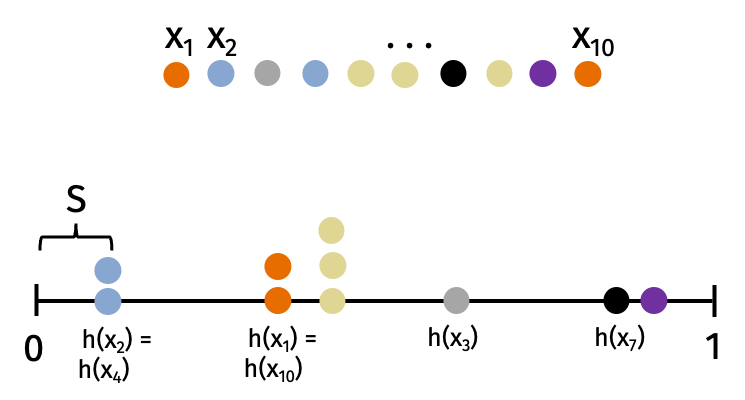
\includegraphics[width=.75\textwidth]{better_minhash_cut.png}
	\end{center}
\end{frame}

\begin{frame}
	\frametitle{visualization}
	\begin{center}
	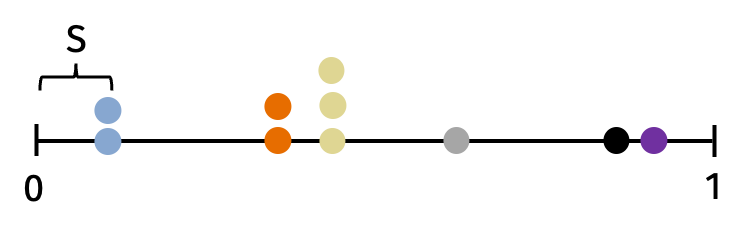
\includegraphics[width=.75\textwidth]{minhash_final_dist.png}
	\end{center}
	\textbf{Important:} If $\mathcal{U} \rightarrow [0,1]$ uniformly at random, we can assume that there are \emph{no collisions}. If we instead used a discrete grid, it would suffice to use a hash table of size $O(D^2)$ or, conservatively, ${O}(|\mathcal{U}|^2)$. \vspace{1em}
	
	We will not do a formal analysis, but roughly how many bits does $S$ takes to store?
\end{frame}





\begin{frame}
	\frametitle{fm analysis}	
	Let $D$ equal the number of distinct elements in our stream.
	\begin{center}
	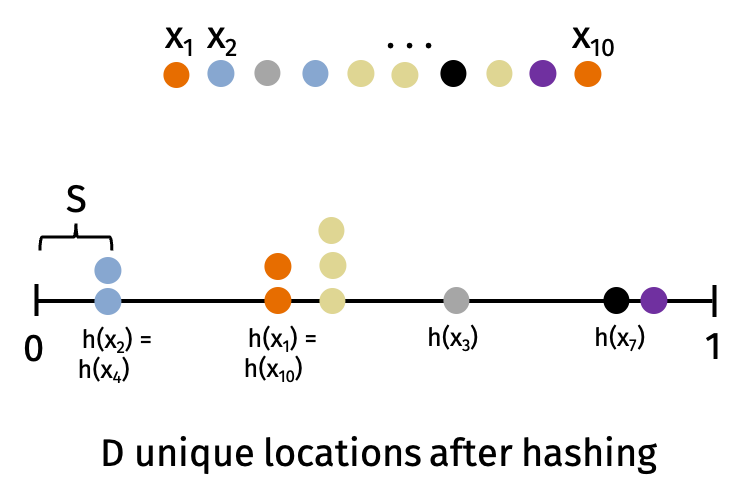
\includegraphics[width=.7\textwidth]{better_minhash.png}
	\end{center}
	\textbf{Intuition:} When $D$ is larger, $S$ will be smaller. Makes sense to return the estimate $\tilde{D} = \frac{1}{S}-1$.
\end{frame}

\begin{frame}
	\frametitle{fm analysis}	
	\textbf{What is $\E S$?}
	\begin{center}
		\uncover<2->{
			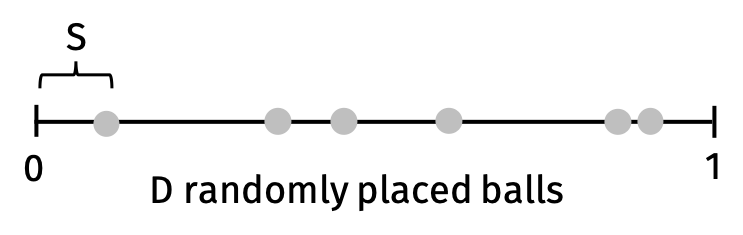
\includegraphics[width=.6\textwidth]{FMimage.png}
		}
	\end{center}
	
	\uncover<3->{
		Let $D$ equal the number of distinct elements in our stream.
		\begin{lemma}
			$\E S = \frac{1}{D + 1}$.
		\end{lemma}
		\vspace{3em}
	}
\end{frame}

\begin{frame}
	\frametitle{the calculus proof}
	\textbf{Proof:} 
	\begin{align*}
		\E[S] &= \int_0^1 \Pr[S \geq \lambda] d\lambda & &\text{Exercise: Why?} \\
		&= \int_0^1 (1-\lambda)^D d\lambda & &\text{} \\
		& = \frac{-(1-\lambda)^{D+1}}{D+1}\Bigm|_{\lambda=0}^1\\
		& = \frac{1}{D+1}
	\end{align*}
\end{frame}



\begin{frame}
	\frametitle{proof ``from the book''}
	$\E[S] = \Pr[(D+1)^\text{st} \text{ item has the smallest hash value}]$.
	\begin{center}
		\uncover<2->{
			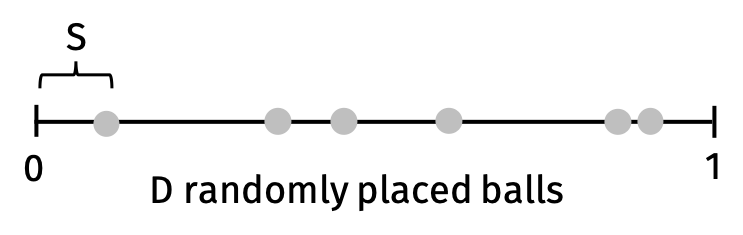
\includegraphics[width=.6\textwidth]{FMimage.png}
		}
	\end{center}
\textbf{Formally, we are using the fact that:}
	\begin{align*}
		&\Pr[A] = \E_{h_1, \ldots, h_D}\left[\Pr\left[A\mid h_1, \ldots, h_D\right]\right]
	\end{align*}
	
\end{frame}

\begin{frame}
	\frametitle{proof ``from the book''}
	$\E[S] = \Pr[(D+1)^\text{st} \text{ item has the smallest hash value}]$.
	\begin{center}
		\uncover<2->{
			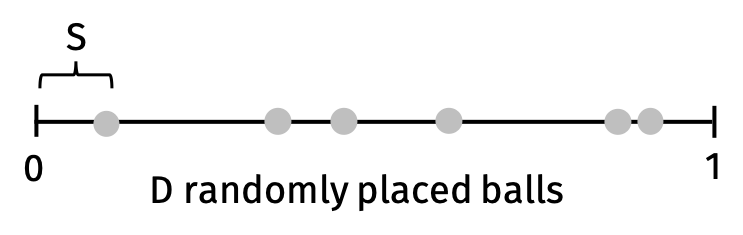
\includegraphics[width=.6\textwidth]{FMimage.png}
		}
	\end{center}
	By symmetry, this equals $\frac{1}{D+1}$ (since every ball is equally likely to be first). 
	
\end{frame}


\begin{frame}
	\frametitle{proving concentration}	
	$\E S = \frac{1}{D + 1}$. \textbf{Estimate:} $\tilde{D} = \frac{1}{S} - 1$. We have for $\epsilon < \frac{1}{2}$:
	
	\begin{center}
	If $(1-\epsilon)\E S \leq S \leq (1+\epsilon)\E S$, then:
	\begin{align*}
	\alert{(1-4\epsilon)D \leq \tilde{D} \leq (1+4\epsilon)D.}
	\end{align*}
	\end{center}
\vspace{10em}

	So, it suffices to show that $S$ concentrates around its mean. I.e. that $|S - \E S| \leq \epsilon\cdot\E S$. We will use Chebyshev's inequality as our concentration bound.
\end{frame}

\begin{frame}
\frametitle{$\epsilon$ manipulation tricks}
\textbf{Recall:}
\begin{align*}
	1+\epsilon \leq \frac{1}{1-\epsilon} \leq 1+ 2\epsilon \text{ for } \epsilon \in [0,.5].
\end{align*}
\begin{align*}
	1-\epsilon \leq \frac{1}{1+\epsilon} \leq 1 - .5\epsilon \text{ for } \epsilon \in [0,1].
\end{align*}
\end{frame}

\begin{frame}
	\frametitle{calculus proof}	
	\begin{lemma}
	$\Var[S] = \E [S^2] - \E[S]^2= \frac{2}{(D+1)(D+2)} - \frac{1}{(D+1)^2} \leq \frac{1}{(D+1)^2}$.
	\end{lemma}
	\textbf{Proof:} 
	\begin{align*}
	\E[S^2] &= \int_0^1 \Pr[S^2 \geq \lambda] d\lambda & &\text{} \\
	&= \int_0^1 \Pr[S \geq \sqrt{\lambda}] d\lambda & &\text{} \\
	&= \int_0^1 (1-\sqrt{\lambda})^D d\lambda & &\text{} \\
	& = \frac{2}{(D+1)(D+2)}& &\text{}
	\end{align*}
	
	\small
	\url{www.wolframalpha.com/input?i=antiderivative+of+\%281-sqrt\%28x\%29\%29\%5ED}
\end{frame}

\begin{frame}
	\frametitle{proof ``from the book''}
	$\E[S^2] = ??$.
	\begin{center}
		\uncover<2->{
			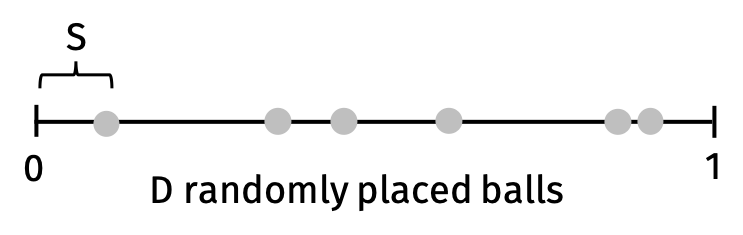
\includegraphics[width=.6\textwidth]{FMimage.png}
		}
	\end{center}
\end{frame}

\begin{frame}
	\frametitle{fm analysis}
	Recall we want to show that, with high probability, $(1-\epsilon) \E[S] \leq S \leq (1-\epsilon) \E[S]$. \vspace{1em}
	\begin{itemize}
		\item $\E[S] = \frac{1}{D+1} = \mu.$ \vspace{.5em}
		\item $\Var[S] \leq \frac{1}{(D+1)^2} = \mu^2$. Standard deviation: $\sigma \leq \mu$. \vspace{.5em}
		\item Want to bound $\Pr[|S - \mu| \geq \epsilon \mu] \leq \delta$. \vspace{.5em}
	\end{itemize}
	
	\textbf{Chebyshev's}: $\Pr[|S - \mu| \geq \epsilon \mu] = \Pr[|S - \mu| \geq \epsilon \sigma] \leq \frac{1}{\epsilon^2}$.
	
	\begin{center}
	\alert{\textbf{Vacuous bound. Our variance is way too high!}}
	\end{center}
\end{frame}


\begin{frame}
	\frametitle{variance reduction}
	\textbf{Trick of the trade:} Repeat many independent trials and take the mean to get a better estimator.
	
	Given i.i.d. (independent, identically distributed) random variables $X_1, \ldots, X_k$ with mean $\mu$ and variance $\sigma^2$, what is:
	\begin{itemize}
		\item $\E\left[\frac{1}{k}\sum_{i=1}^k X_i\right] = $
		\vspace{1em}
		\item $\Var\left[\frac{1}{k}\sum_{i=1}^k X_i\right] = $
	\end{itemize} 
\end{frame}

\begin{frame}
	\frametitle{fm analysis}
	Using independent hash functions, maintain $k$ independent sketches $S_1, \ldots, S_k$.
\vspace{-1em}
\begin{center}
	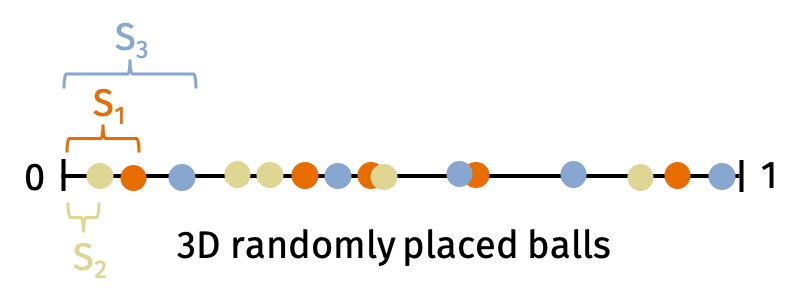
\includegraphics[width=.7\textwidth]{improvedFM.png}
\end{center}

\vspace{-1em}	
\textbf{Flajolet–Martin}:
		\begin{itemize}
			\item Choose $k$ random hash function $h_1, \ldots, h_k: \mathcal{U} \rightarrow [0,1]$.
			\item $S_1 = 1, \ldots, S_k = 1$ 
			\item For $i = 1, \ldots, n$
			\begin{itemize}
				\item $S_j \leftarrow \min(S_j, h_j(x_i))$ for all $j \in 1, \ldots, k$.
			\end{itemize} 
			\item $S = (S_1 + \ldots + S_k)/k$
			\item Return: $\frac{1}{S} - 1$
		\end{itemize}
\end{frame}

\begin{frame}
	\frametitle{fm analysis}
	\textbf{1 estimator}:
	\begin{itemize}
		\item $\E[S] = \frac{1}{D+1} = \mu.$
		\item $\Var[S] = \mu^2$
	\end{itemize}
	\textbf{$k$ estimators}:
	\begin{itemize}
		\item $\E[S] = \frac{1}{D+1} = \mu.$
		\item $\Var[S] \leq  \mu^2/k$
		\item By Chebyshev, $\Pr[|S - \E S| \geq c \mu/\sqrt{k}] \leq \frac{1}{c^2}$.
	\end{itemize}

	Setting $c = 1/\sqrt{\delta}$ and $k = \frac{1}{\epsilon^2\delta}$ gives:
	\begin{align*}
		\Pr[|S - \mu| \geq \epsilon \mu] \leq \delta.
	\end{align*}


\textbf{Total space complexity}: $\alert{O\left(\frac{1}{\epsilon^2\delta}\right)}$ to estimate distinct elements up to error $\epsilon$ with success probability $1-\delta$.
\end{frame}

\begin{frame}[t]
	\frametitle{fm analysis}
	\textbf{Total space complexity}: $\alert{O\left(\frac{1}{\epsilon^2\delta}\right)}$ to estimate distinct elements up to error $\epsilon$ with success probability $1-\delta$.
	
	\begin{itemize}
		\item Recall that to ensure $(1-\bar{\epsilon}) D \leq \frac{1}{S} - 1 \leq (1+\bar{\epsilon}) D$, we needed  $|S - \mu| \leq \frac{\bar{\epsilon}}{4} \mu$. 
		\item So apply the result from the previous slide with $\epsilon = \bar{\epsilon}/4$. 
		\item Need to store $k = \frac{1}{\epsilon^2\delta} = \frac{1}{(\bar{\epsilon}/4)^2\delta} = \frac{16}{\epsilon^2\delta}$ counters.
	\end{itemize}
\end{frame}

\begin{frame}
	\frametitle{note on failure probability}
	$\alert{O\left(\frac{1}{\epsilon^2\delta}\right)}$ space is an impressive bound:
	\begin{itemize}
		\item $1/\epsilon^2$ dependence cannot be improved.
		\item No linear dependence on number of distinct elements $D$.\footnote{Technically, if we account for the bit complexity of storing $S_1, \ldots, S_k$ and the hash functions $h_1, \ldots, h_k$, the space complexity is $O\left(\frac{\log D}{\epsilon^2\delta}\right)$.}
		\item But... $1/\delta$ dependence is not ideal. For $95\%$ success rate, pay a $\frac{1}{5\%} = 20$ factor overhead in space. 
	\end{itemize}
We can get a better bound depending on $O(\log(1/\delta))$ using \emph{exponential tail bounds.} We will see next lecture.
\end{frame}

\begin{frame}
	\frametitle{distinct elements in practice}
	In practice, we cannot hash to real numbers on $[0,1]$. Instead, map to bit vectors.
	
	\textbf{Real Flajolet-Martin / HyperLogLog:}
	\begin{columns}
		\begin{column}{.4\textwidth}
			\begin{center}
				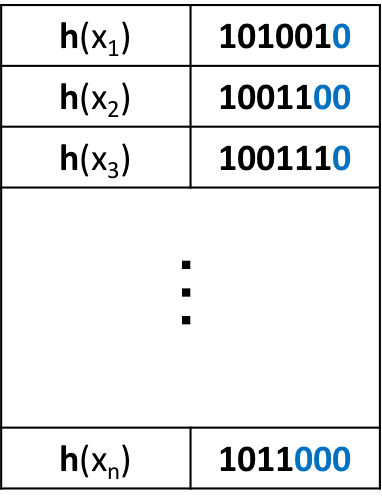
\includegraphics[width=.7\textwidth]{loglog2.png}
			\end{center}
		\end{column}
		\begin{column}{.6\textwidth}
				\begin{itemize}
					\item Estimate \# distinct elements based on maximum number of trailing zeros $\bv m$.
					\item The more distinct hashes we see, the higher we expect this maximum to be.
				\end{itemize}
		\end{column}
	\end{columns}
	\begin{center}
	\end{center}
\end{frame}

\begin{frame}
	\frametitle{loglog space}
	\textbf{Total Space:} $O \left (\frac{\log \log D}{\epsilon^2} + \log D \right )$ for an $\epsilon$ approximate count.
	
	\small ``Using an auxiliary memory smaller than the size of this abstract, the LogLog algorithm makes it possible to estimate in a single pass and within a few percents the number of different words in the whole of Shakespeare’s works.'' -- Flajolet, Durand.
	
	
	\vspace{1em}
	\uncover<3->{
		Using HyperLogLog to count $1$ billion distinct items with $2\%$ accuracy:
		\begin{align*}
			\text{space used } &= O \left (\frac{\log \log D}{\epsilon^2} + \log D \right )\\ \uncover<2->{&= \frac{1.04 \cdot \lceil \log_2 \log_2 D\rceil}{\epsilon^2} + \lceil \log_2 D \rceil \text{ bits}\\}
			\uncover<3->{&= \frac{1.04 \cdot 5}{.02^2} + 30 = 13030\text{ bits} \approx \alert{1.6\ kB}!}
		\end{align*}
	}
\end{frame}

\begin{frame}
	\frametitle{hyperloglog in practice}
	\begin{center} 
		Although, to be fair, storing a dictionary with $1$ billion bits only takes 125 megabytes. Not tiny, but not unreasonable.
		
		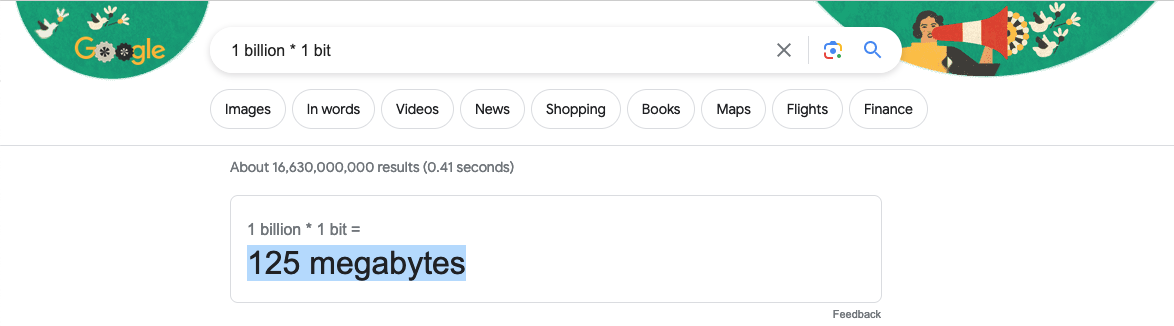
\includegraphics[width=\textwidth]{google_bit_calculations.png}
	\end{center}
	These estimators become more important when you want to count \emph{many} different things (e.g., a software company tracking clicks on 100s of UI elements).
\end{frame}

\begin{frame}
	\frametitle{distributed distinct elements}
	Also very important in distributed settings. 
	\begin{center}
		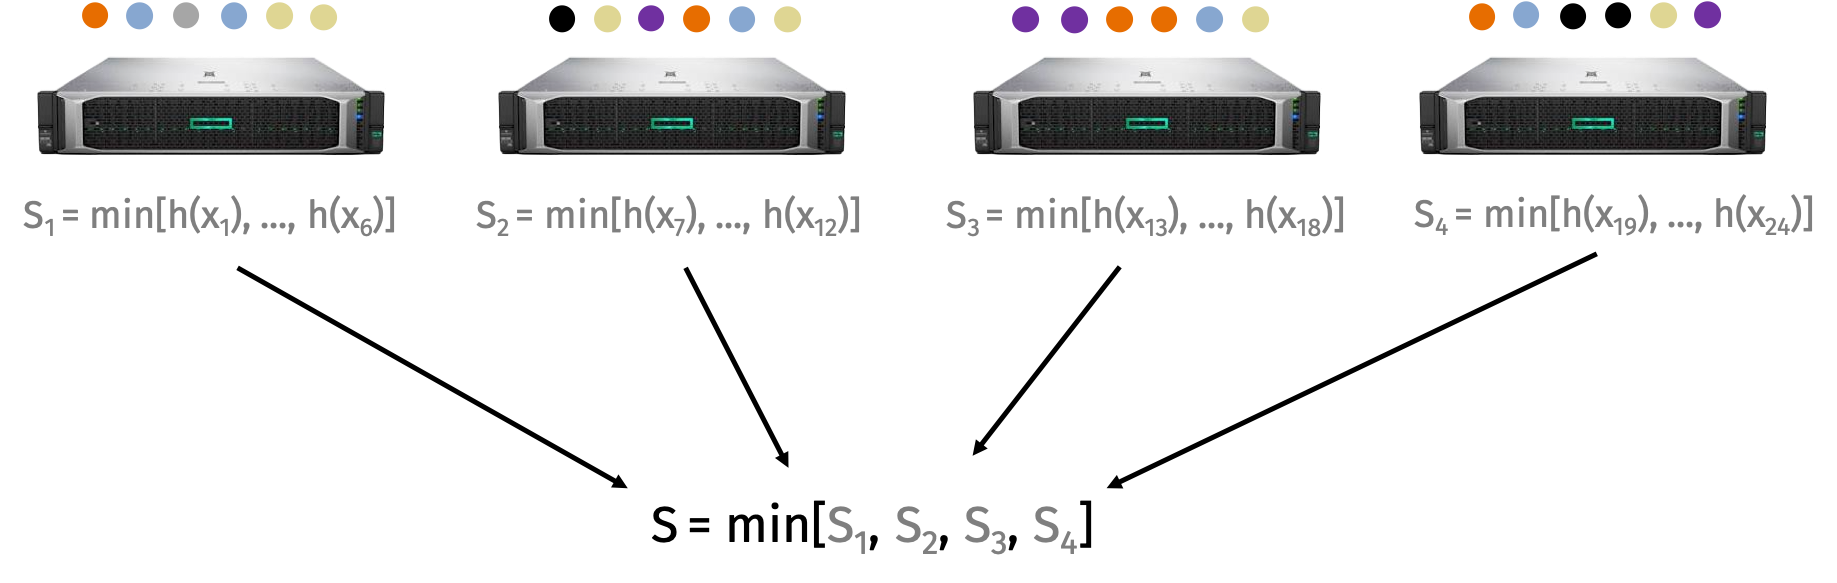
\includegraphics[width=\textwidth]{dist_min_hash.png}
	\end{center}

	Distinct elements summaries are ``mergeable''. No need to share lists of distinct elements if those elements are stored on different machines. Just share minimum hash value.
\end{frame}

\begin{frame}
	\frametitle{hyperloglog in practice}
	\small
	\textbf{Implementations:} Google PowerDrill, Facebook Presto, Twitter Algebird, Amazon Redshift.
	
	\textbf{Use Case:} Exploratory SQL-like queries on tables with $100$'s of billions of rows.
	\begin{itemize}
		\item \alert{Count} number of \alert{distinct} users in Germany that  made at least one search containing the word `auto' in the last month.
		\item \alert{Count} number of \alert{distinct} subject lines in emails sent by users that have registered in the last week, in comparison to number of emails sent overall (to estimate rates of spam accounts).
		% \item \alert{Count} number of \alert{distinct} zip codes in which at least one search has been made for blah
	\end{itemize}
	\uncover<2->{
		\begin{center}
			\textbf{Answering a query requires a (distributed) linear scan over the database: \emph{2 seconds} in Google's distributed implementation.}
			
				\textbf{\alert{Google Paper: ``Processing a Trillion Cells per Mouse Click''}}
		\end{center}
	}
\end{frame}

%\begin{frame}
%	\frametitle{hyperloglog in practice}
%	\textbf{Google Paper: ``Processing a Trillion Cells per Mouse Click''}
%	
%	``The system has been in production since end of 2008 and
%	was made available for internal users across all of Google
%	mid 2009. Each month it is used by more than 800 users
%	sending out about 4 million SQL queries. \textbf{\alert{After a hard day’s
%			work, one of our top users has spent over 6 hours in the
%			UI, triggering up to 12 thousand queries.}} When using our
%	column-store as a backend, this may amount to scanning as
%	much as 525 trillion cells in (hypothetical) full scans.''
%\end{frame}

% \begin{frame}[standout]
% 	\begin{center}
% 		break
% 	\end{center}
% \end{frame}



\end{document} 








